\documentclass[10pt]{article}
\usepackage[utf8]{inputenc}
\usepackage[T1]{fontenc}
\usepackage{amsmath}
\usepackage{amsfonts}
\usepackage{amssymb}
\usepackage[version=4]{mhchem}
\usepackage{stmaryrd}
\usepackage{graphicx}
\usepackage[export]{adjustbox}
\graphicspath{ {./images/} }

\begin{document}
You are allowed to use a scientific calculator on this assessment. All answers must be completely simplified to earn full credit.

\begin{enumerate}
  \item If $f(x)=-3 x^{3}(3-2 x)^{3}(x+5)$, use a sketch of $f(x)$ to find all interval(s) for which $f(x)>0$. $(2 \mathrm{Pts})$
  \item The graph of the polynomial function $g(x)$ is shown below. If $x^{2}$ is a factor of $g(x)$ in factored form, and $x=1+i$ is a root of $g(x)$, what is the minimum possible degree of $g(x)$ ? ( 1 pt )\\
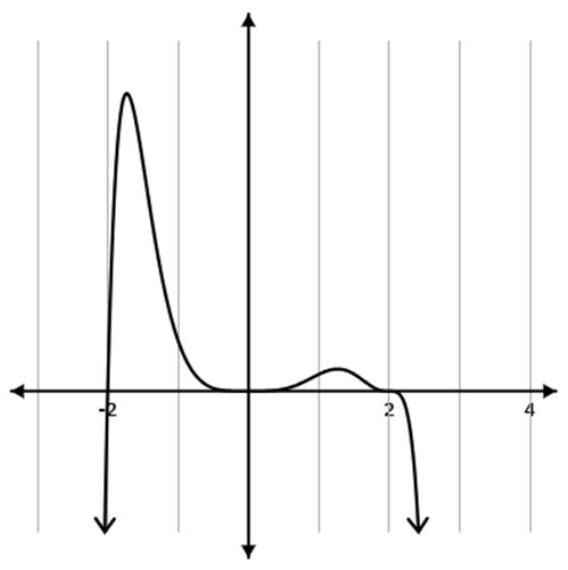
\includegraphics[max width=\textwidth, alt={}, center]{0749201f-ab72-4161-b8a4-311901f79ff0-01_570_568_472_1310}
\end{enumerate}

Answer: $\_\_\_\_$\\
3. The graph of $h(x)$ is shown below. Which of the following could be the equation of $h(x)$ ? (1 pt)\\
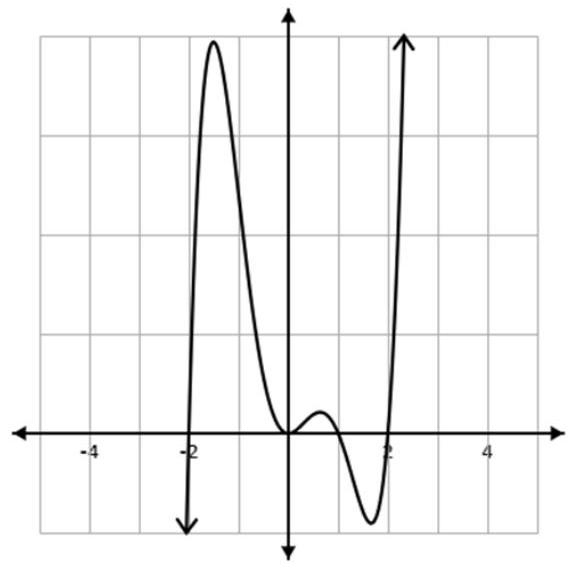
\includegraphics[max width=\textwidth, alt={}, center]{0749201f-ab72-4161-b8a4-311901f79ff0-01_570_579_1293_352}\\
a) $2 x^{2}(x-1)\left(x^{2}-4\right)$\\
b) $\quad 2 x^{2}(x-1)\left(x^{2}+4\right)$\\
c) $\quad 2 x^{2}(x+1)\left(x^{2}-4\right)$\\
d) $2 x^{2}(x+1)\left(x^{2}+4\right)$\\
4. A polynomial function $m(x)$ has real roots at $a, b$, and $c$ such that $-10 \leq a<b<c \leq 10$. $m(x)$ has no roots with an imaginary unit. The root $b$ has a multiplicity of 4, and it is known that $m(-11)=-m(10)=3$. Which of the following must be true? Select all that apply. (3 pts)\\
a) $m(9)<0$\\
b) $a$ and $c$ cannot have the same multiplicity\\
c) $m(x)$ has a negative leading coefficient\\
d) $a$ has an odd multiplicity, and $c$ has an even multiplicity\\
e) $c \neq 10$\\
f) $\quad \lim _{x \rightarrow-\infty} m(x)=-\infty$\\
5. Expand $(x-2 i)^{4}$ (3 pts)\\
6. Use the function $f(x)=27 x^{5}+36 x^{4}-6 x^{3}+42 x^{2}-33 x+6$ for the following questions.\\
a) State the end behavior of $f(x)$ as $x$ increases without bound. Write your answer in limit notation. (3 pts)\\
b) Given that $f\left(\frac{1}{3}\right)=0$, and that $f(x)$ has 2 roots that contain imaginary units, find all roots of $f(x)$ and their multiplicities. (5 pts)

\begin{center}
\begin{tabular}{|c|c|}
\hline
Root & Multiplicity \\
\hline
 &  \\
\hline
 &  \\
\hline
 &  \\
\hline
 &  \\
\hline
\end{tabular}
\end{center}

c) Graph $f(x)$. Be sure to include the correct end behavior, intercepts, and behavior at the roots. (4 pts)\\
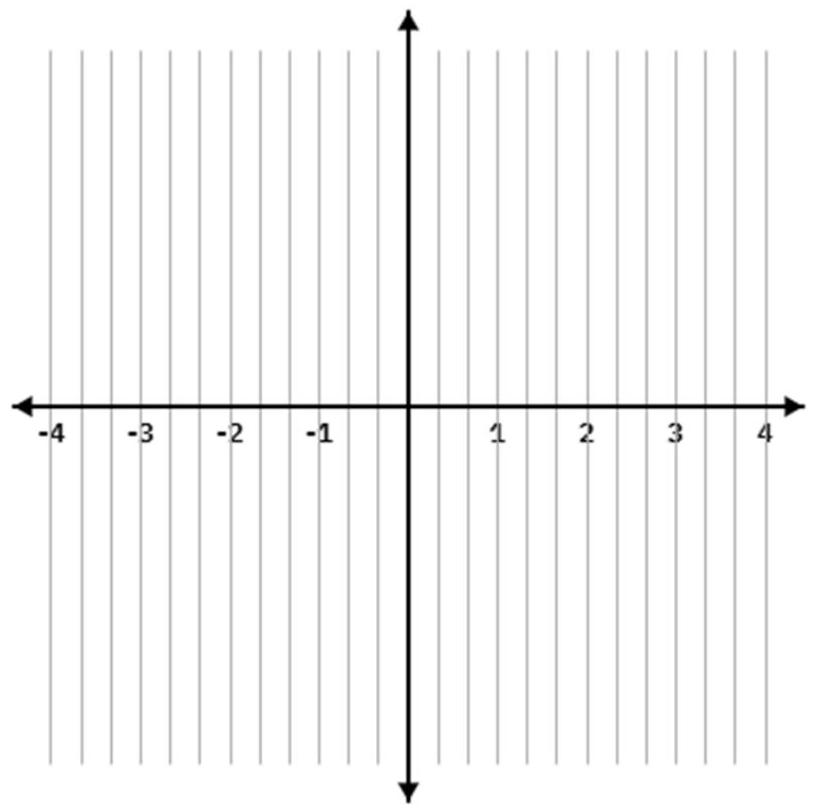
\includegraphics[max width=\textwidth, alt={}, center]{0749201f-ab72-4161-b8a4-311901f79ff0-02_811_816_1851_605}\\
7. Solve the equation $x^{3}-6 x^{2}-10 x+10=15 x-x^{3}-7 x^{2}-2$. ( 4 pts)\\
8. Given that $x=i$ is a root of $f(x)=3 x^{4}+9 x^{3}+10 x^{2}+a x+7$, find the value of $a$. (3 pts)\\
9. The expansion of $\left(2 x^{2}-3 y^{4}\right)^{9}$ contains the term $a x^{8} y^{k}$. Find the values of $a$ and $k$. Both answers should be numeric. Your answer cannot contain factorials. (3 points)

You are allowed to use a scientific calculator on this assessment. All answers must be completely simplified to earn full credit.

\begin{enumerate}
  \item If $f(x)=3 x^{2}(4-3 x)^{3}(x-5)$, use a sketch of $f(x)$ to find all interval(s) for which $f(x)>0$. (2 pts)
  \item The graph of the polynomial function $g(x)$ is shown below. If $x^{4}$ is a factor of $g(x)$ in factored form, and $x=1+i$ is a root of $g(x)$, what is the minimum possible degree of $g(x)$ ? ( 1 pt )\\
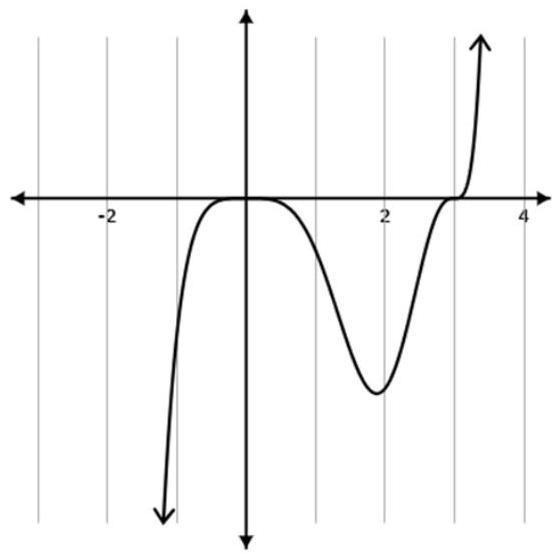
\includegraphics[max width=\textwidth, alt={}, center]{0749201f-ab72-4161-b8a4-311901f79ff0-05_557_560_485_1327}
\end{enumerate}

Answer: $\_\_\_\_$\\
3. The graph of $h(x)$ is shown below. Which of the following could be the equation of $h(x)$ ? (1 pt)\\
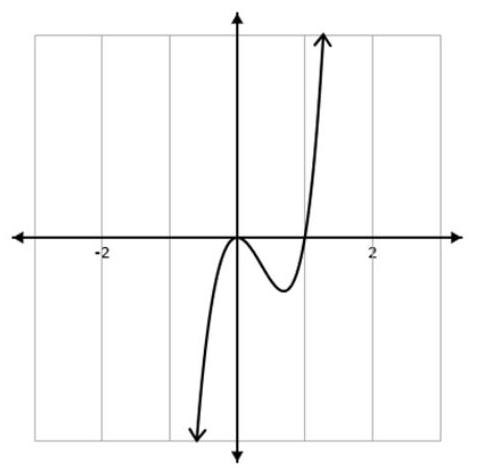
\includegraphics[max width=\textwidth, alt={}, center]{0749201f-ab72-4161-b8a4-311901f79ff0-05_474_478_1327_395}\\
a) $2 x^{2}(x-1)\left(x^{2}-4\right)$\\
b) $\quad 2 x^{2}(x-1)\left(x^{2}+4\right)$\\
c) $\quad 2 x^{2}(x+1)\left(x^{2}-4\right)$\\
d) $2 x^{2}(x+1)\left(x^{2}+4\right)$\\
4. A polynomial function $m(x)$ has real roots at $a, b$, and $c$ such that $-10 \leq a<b<c \leq 10$. $m(x)$ has no roots with an imaginary unit. The root $a$ has a multiplicity of 4 , and it is known that $m(-11)=m(10)=3$. Which of the following must be true? Select all that apply. (3 pts)\\
a) $m(9)>0$\\
b) $\quad b$ and $c$ have the same multiplicity\\
c) $m(x)$ has a negative leading coefficient\\
d) If $b$ has an odd multiplicity, then $c$ has an odd multiplicity\\
e) $c \neq 10$\\
f) $\lim _{x \rightarrow-\infty} m(x)=\infty$\\
5. Expand $(x-3 i)^{4}$ (3 pts)\\
6. Use the function $f(x)=4 x^{5}+8 x^{4}+25 x^{3}+75 x^{2}-99 x+27$ for the following questions.\\
a) State the end behavior of $f(x)$ as $x$ increases without bound. Write your answer in limit notation. (3 pts)\\
b) Given that $f\left(\frac{1}{2}\right)=0$, and that $f(x)$ has 2 roots that contain imaginary units, find all roots of $f(x)$ and their multiplicities. (5 pts)

\begin{center}
\begin{tabular}{|l|l|}
\hline
Root & Multiplicity \\
\hline
 &  \\
\hline
 &  \\
\hline
 &  \\
\hline
 &  \\
\hline
\end{tabular}
\end{center}

c) Graph $f(x)$. Be sure to include the correct end behavior, intercepts, and behavior at the roots. (4 pts)\\
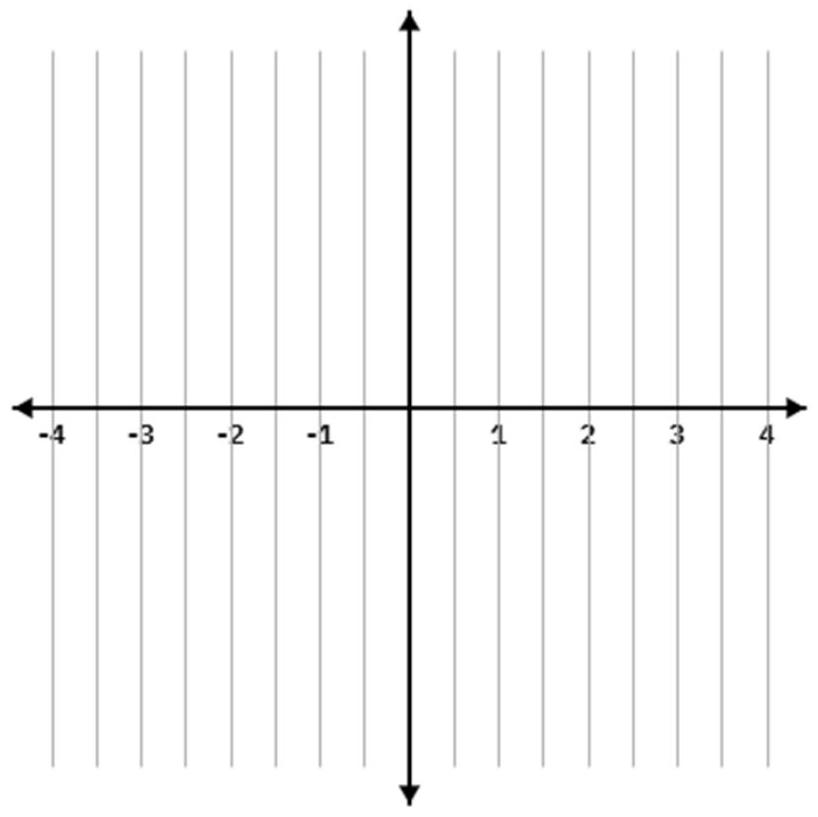
\includegraphics[max width=\textwidth, alt={}, center]{0749201f-ab72-4161-b8a4-311901f79ff0-06_817_818_1845_603}\\
7. Solve the equation $2 x^{3}+6 x^{2}-10 x+8=5 x^{2}+3 x+2$. ( 4 pts)\\
8. Given that $x=2 i$ is a root of $f(x)=5 x^{4}-2 x^{3}+27 x^{2}+a x+28$, find the value of $a$. ( 3 pts )\\
9. The expansion of $\left(3 x^{2}-2 y^{4}\right)^{9}$ contains the term $a x^{4} y^{k}$. Find the values of $a$ and $k$. Both answers should be numeric. Your answer cannot contain factorials. (3 points)

You are allowed to use a scientific calculator on this assessment. All answers must be completely simplified to earn full credit.

\begin{enumerate}
  \item If $f(x)=-3 x^{3}(2 x-3)^{2}(x+5)$, use a sketch of $f(x)$ to find all interval(s) for which $f(x) \leq 0$. (2 pts)
  \item The graph of the polynomial function $g(x)$ is shown below. If $x^{2}$ is a factor of $g(x)$ in factored form, and $x=2 i$ is a root of $g(x)$, what is the minimum possible degree of $g(x)$ ? (1 point)\\
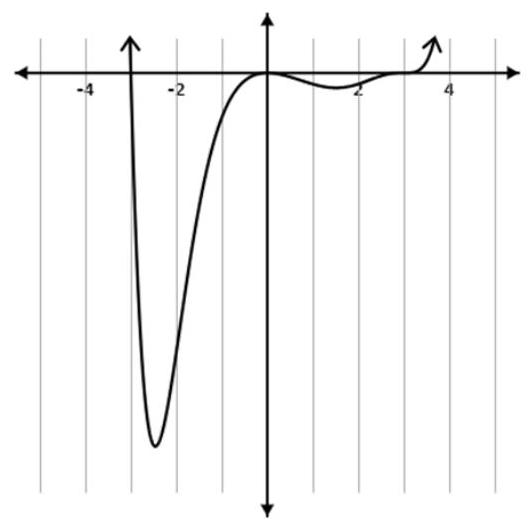
\includegraphics[max width=\textwidth, alt={}, center]{0749201f-ab72-4161-b8a4-311901f79ff0-09_530_532_489_1314}
\end{enumerate}

Answer: $\_\_\_\_$\\
3. The graph of $h(x)$ is shown below. Which of the following could be the equation of $h(x)$ ? (1 pt)\\
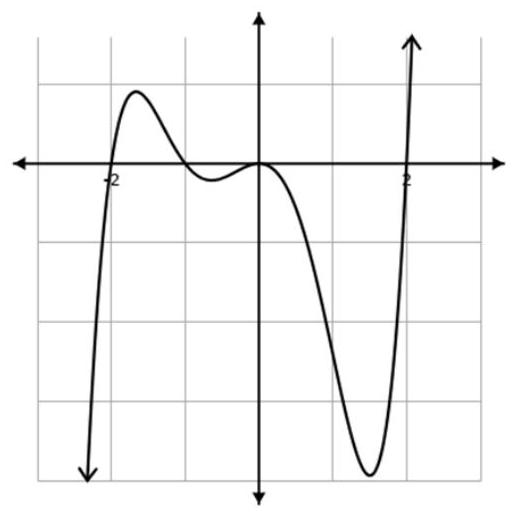
\includegraphics[max width=\textwidth, alt={}, center]{0749201f-ab72-4161-b8a4-311901f79ff0-09_519_519_1314_403}\\
a) $2 x^{2}(x-1)\left(x^{2}-4\right)$\\
b) $2 x^{2}(x-1)\left(x^{2}+4\right)$\\
c) $\quad 2 x^{2}(x+1)\left(x^{2}-4\right)$\\
d) $2 x^{2}(x+1)\left(x^{2}+4\right)$\\
4. A polynomial function $m(x)$ has real roots at $a, b$, and $c$ such that $-8 \leq a<b<c \leq 11 . m(x)$ has no roots with an imaginary unit. The root $c$ has a multiplicity of 3 , and it is known that $m(-11)=-m(12)=-3$. Which of the following must be true? Select all that apply. (3 pts)\\
a) $m(-9)<0$\\
b) $a$ and $b$ cannot have the same multiplicity\\
c) $m(x)$ has a negative leading coefficient\\
d) If $a$ has an odd multiplicity, then $b$ has an even multiplicity\\
e) $c \neq 11$\\
f) $\quad \lim _{x \rightarrow-\infty} m(x)=-\infty$\\
5. Expand $(2 x-i)^{4}$ (3 pts)\\
6. Use the function $f(x)=9 x^{5}-30 x^{4}+37 x^{3}-38 x^{2}+28 x-8$ for the following questions.\\
a) State the end behavior of $f(x)$ as $x$ increases without bound. Write your answer in limit notation. (3 pts)\\
b) Given that $f\left(\frac{2}{3}\right)=0$, and that $f(x)$ has 2 roots that contain imaginary units, find all roots of $f(x)$ and their multiplicities. (5 pts)

\begin{center}
\begin{tabular}{|c|c|}
\hline
Root & Multiplicity \\
\hline
 &  \\
\hline
 &  \\
\hline
 &  \\
\hline
 &  \\
\hline
\end{tabular}
\end{center}

c) Graph $f(x)$. Be sure to include the correct end behavior, intercepts, and behavior at the roots. (4 pts)\\
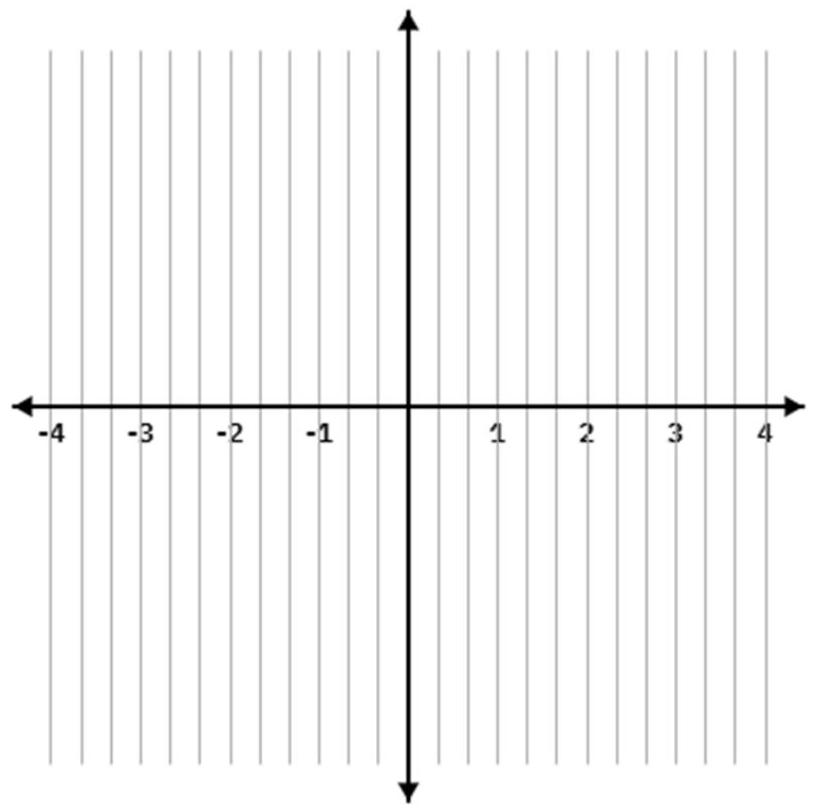
\includegraphics[max width=\textwidth, alt={}, center]{0749201f-ab72-4161-b8a4-311901f79ff0-10_811_816_1851_605}\\
7. Solve the equation $6 x^{3}+4 x^{2}-23 x+9=3 x^{3}+3 x^{2}-3 x-3$. ( 4 pts)\\
8. Given that $x=3 i$ is a root of the function $f(x)=3 x^{4}-5 x^{3}+29 x^{2}+a x+18$, find the value of $a$. (3 pts)\\
9. The expansion of $\left(2 x^{2}-5 y^{4}\right)^{9}$ contains the term $a x^{12} y^{k}$. Find the values of $a$ and $k$. Both answers should be numeric. Your answer cannot contain factorials. (3 points)


\end{document}